\chapterimage{01_Uvod.jpg} % Chapter heading image

\chapter{Uvod}

\section{Optika}
Optika je veda o svetlobi, pri čemer različne veje optike svetlobo
obravnavajo na različne načine. Najpreprostejši pristop je 
opis svetlobe z ravnimi žarki, kar sodi v okvir geometrijske optike. 
Poglavitna pojava v tem približku sta lom in odboj, 
zato lahko z geometrijsko optiko opišemo preslikavo z lečo ali 
odboj na zrcalu in pojasnimo delovanje optičnih naprav, kakršne so 
lupa, mikroskop, teleskop ali oko. Geometrijsko optiko bomo na kratko
obravnavali takoj za uvodom.

Valovna optika obravnava svetlobo kot elektromagnetno valovanje. Preprostejši
pristop sloni na skalarni obravnavi jakosti električnega polja, kar zadošča
za opis interference, uklona, absorpcije v snovi in podobnih pojavov. Splošnejši
zapis je vektorski, v katerem upoštevamo tudi polarizacijo svetlobe in 
z njo povezane pojave. V večini poglavij bomo svetlobo opisali
z valovno optiko. 

V zadnjem poglavju se bomo odklonili od klasične optike in
predstavili uvod v kvantno optiko. Svetlobe ne bomo več obravnavali  
kot valovanje, temveč bo sestavljena iz potujočih kvantov energije, tako 
imenovanih fotonov. Ta pristop je pomemben predvsem  
pri natančnejši obravnavi interakcije svetlobe s snovjo, opisu sevanja 
črnega telesa in razlagi delovanja laserjev. Še splošnejši pristop
s kvantno elektrodinamiko presega okvir te knjige. 

\section{Kratek zgodovinski pregled}\index{Zgodovina optike}
Začetki optike sežejo zelo daleč v zgodovino.\footnote{~Glej 
npr. B. Vohnsen, Phys. Scr. {\bf T109}, 75 (2004); 
E. Hecht, {\it Optics}, peta izdaja, Pearson (2017) ali
M. Born in E. Wolf, {\it Principles of Optics}, sedma izdaja, 
Cambridge University Press (1999).} Najstarejša najdena ogledala, 
stara skoraj 4000~let, so odkrili v grobnicah starih Egipčanov. 
Izdelana so bila iz bakra ali brona, nato pa skrbno polirana in okrašena. 
Bolj znanstveno so se obravnave optike lotili starogrški
misleci, med drugim Pitagora\footnote{~Grški 
matematik, okoli 570 -- okoli 495 pr.\,n.\,št.}, Platon\footnote{~Grški 
filozof, 427--347 pr.\,n.\,št.} in Aristotel\footnote{~Grški 
filozof, 384--322 pr.\,n.\,št.}, ki so se\index{Pitagora}\index{Platon}\index{Aristotel}
ukvarjali predvsem s tem, kako nek predmet vidimo in zaznamo. Prevladovala
je teza, da oko oddaja žarke, ki vpadajo na predmete.
Evklid\footnote{~Grški 
matematik, okoli 365--275 pr.\,n.\,št.} \index{Evklid} je okoli leta $300$~pr.\,n.\,št.\,ugotovil, 
da se svetloba širi v ravni črti in zapisal odbojni zakon. Heron\footnote{~Grški 
znanstvenik Heron iz Aleksandrije, okoli 20 -- okoli 100.} je ugotovitve združil
v pravilo, da svetloba med dvema točkama potuje po najkrajši poti.\index{Heron}
Stari Grki -- in kasneje stari Rimljani -- so poznali krogelna zrcala, 
uporabljali zbiralne leče za netenje ognja, 
proučevali lom svetlobe ob prehodu iz zraka v vodo ali steklo
in uporabljali steklene bučke, napolnjene z vodo, za povečavo slik.

Z zatonom Zahodnega rimskega cesarstva se je razvoj znanosti pretežno 
preselil v arabski svet. Najpomembnejši predstavnik je zagotovo 
Alhazen\footnote{~Arabski znanstvenik Abu 
Ali al-Hasan ibn al-Haitam ali krajše Ibn al-Haitam, 965--1041.}, \index{Alhazen}
ki je okoli leta 1000 napisal obširno knjigo v sedmih delih
z naslovom {\it Knjiga o optiki}. 
V njej je med drugim podrobno opisal lom svetlobe in delovanje sferičnih,
eliptičnih ter paraboličnih zrcal in leč. Postavil je model, 
po katerem je vsaka točka osvetljenega telesa izvor
ravnih žarkov svetlobe, ki jih zaznamo, ko padejo v oko. 
Zapisal je tudi tezo, da svetloba med dvema točkama potuje po najhitrejši poti.

V srednjem veku v Evropi optiki kot znanosti niso posvečali veliko
pozornosti, so pa uporabljali preproste optične naprave. 
Konec trinajstega stoletja so alkimisti izdelovali ogledala, 
tako da so na steklo nanašali zlitine kositra in živega srebra, 
italijanski steklarski mojstri pa so že izdelovali korekcijske leče 
oziroma očala. Roger Bacon\footnote{~Angleški učenjak Roger Bacon, 1214--1294.}\index{Bacon, Roger}
je daljnovidnim za izboljšanje vida priporočal uporabo zbiralnih leč, 
od začetka šestnajstega stoletja pa so uporabljali tudi razpršilne leče
za izboljšanje vida kratkovidnih. Vendar se o tem, kako leče delujejo, 
niso spraševali. 

\begin{figure}[ht]
\centering
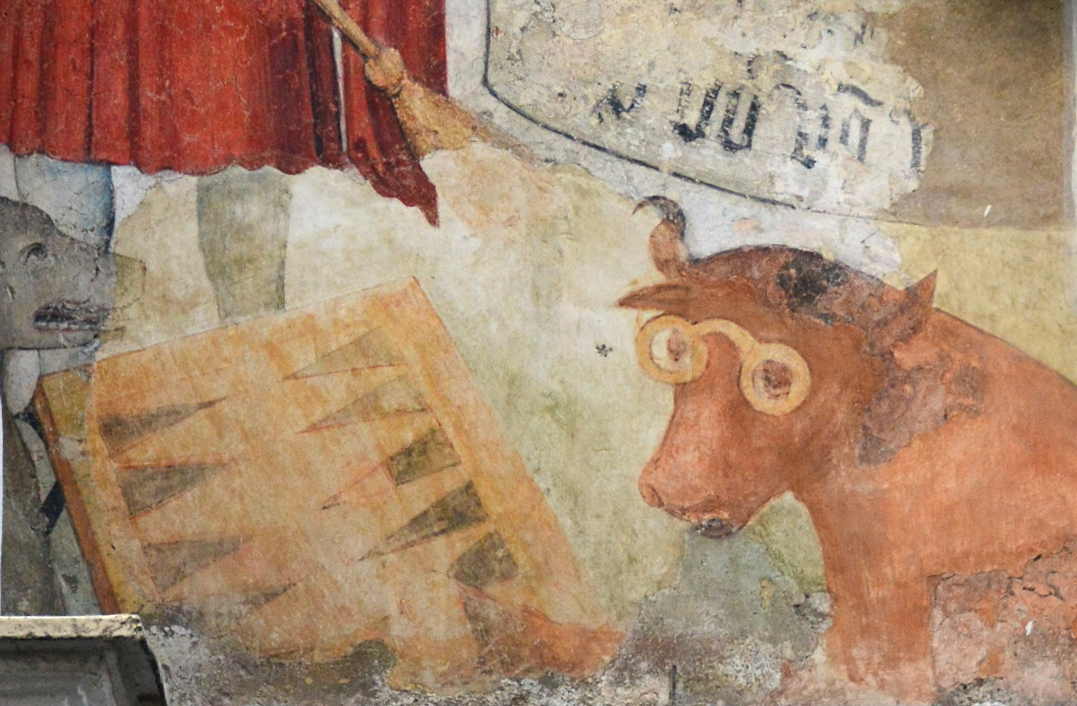
\includegraphics[width=85truemm]{slike/01_Dunaj.jpg}
\caption{Freska na Dunaju (17. stoletje) prikazuje kravo z očali.}
\label{fig:01_Dunaj}
\end{figure}

Odgovore na vprašanja, kako deluje leča in zakaj očala izboljšajo vid, je podal
Kepler\footnote{~Nemški astronom Johannes Kepler, 1571--1630.} leta 1611.\index{Kepler, Johannes}
Poleg tega je odkril totalni odboj svetlobe in zapisal lomni zakon za majhne kote.
Na splošno je začetek sedemnajstega stoletja predstavljal preporod optike. 
V tem času so na Nizozemskem začeli izdelovati prve daljnoglede oziroma
teleskope, sestavljene iz dveh leč:
najprej zbiralne in razpršilne, pozneje pa iz dveh zbiralnih leč. 
Nizozemski znanstvenik Snell\footnote{~Nizozemski matematik in astronom Willebrord 
Snell van Royen, 1580--1626.} je zapisal lomni zakon v današnji obliki in \index{Snell van Royen, Willebrord}
marsikje zato lomni zakon še vedno imenujejo po njem. Pomemben teorem, s katerim
bomo tudi mi začeli obravnavno optike v naslednjem poglavju, je postavil 
Fermat\footnote{~Francoski pravnik in matematik Pierre de Fermat, 1601--1665.} \index{Fermat, Pierre de}
leta 1657. Teorem pravi, da svetloba med dvema točkama potuje po tisti poti, 
po kateri do cilja pride najhitreje.\index{Fermatov teorem}

V drugi polovici sedemnajstega stoletja so Grimaldi\footnote{~Italijanski \index{Grimaldi, Francesco}
fizik in astronom Francesco Maria Grimaldi, 1618--1663.}, Huygens\footnote{~Nizozemski \index{Huygens, Christiaan}
astronom in matematik Christiaan Huygens, 1629--1695.} in Hooke\footnote{~Angleški \index{Hooke, Robert}
fizik in zdravnik Robert Hooke, 1635--1703.} proučevali uklon. Ugotovili so, da se 
svetloba širi tudi v območje sence in da torej svetloba ne potuje vedno 
povsem naravnost. Predvsem Huygens je, po podobnosti z zvokom, verjel v 
valovno naravo svetlobe. Širjenje svetlobe je pojasnil z načelom, 
po katerem vsako točko, na katero vpade valovna motnja, obravnavamo 
kot nov točkast izvor, iz katerega se motnja širi v obliki krogelnih valov. 
S tem pristopom je lahko pojasnil odboj in lom na meji dveh sredstev. Sklepal je, da
se svetloba v gostejših snoveh upočasni.
Opazoval in pojasnil je razklon svetlobe na dva žarka v kristalu kalcita 
in s tem odkril polarizacijo svetlobe. Huygens je sodeloval tudi pri 
prvih meritvah hitrosti svetlobe. 

Že od antičnih časov so vedeli, da
je hitrost svetlobe ali zelo velika ali celo neskončna. Prve uspešne kvantitativne
meritve je naredil R\o{}mer\footnote{~Danski astronom \index{R\o{}mer, Ole Christensen}
Ole Christensen R\o{}mer, 1644--1710.} leta 1676, ko je z natančnim opazovanjem 
mrkov Jupitrovih lun ugotovil, da je hitrost svetlobe končna. Hitrost svetlobe je
ocenil na $230\,\,000~\si{km/s}$.

K razumevanju svetlobe je pomembno prispeval Newton\footnote{~Angleški \index{Newton, Sir Isaac}
fizik in matematik Sir Isaac Newton, 1643--1727.}, ko je v letih 1666--72 
izvajal poskuse s stekleno prizmo. S prizmo je razklonil sončno svetlobo v
mavrico in s tem pokazal, da je bela svetloba sestavljena 
iz svetlob različnih barv. Na splošno je bil pristaš teorije, da je 
svetloba sestavljena iz delcev. Ker je bil v tistih časih 
Newton nesporna avtoriteta na področju fizike, je ta pogled obveljal.
\begin{figure}[ht]
\centering
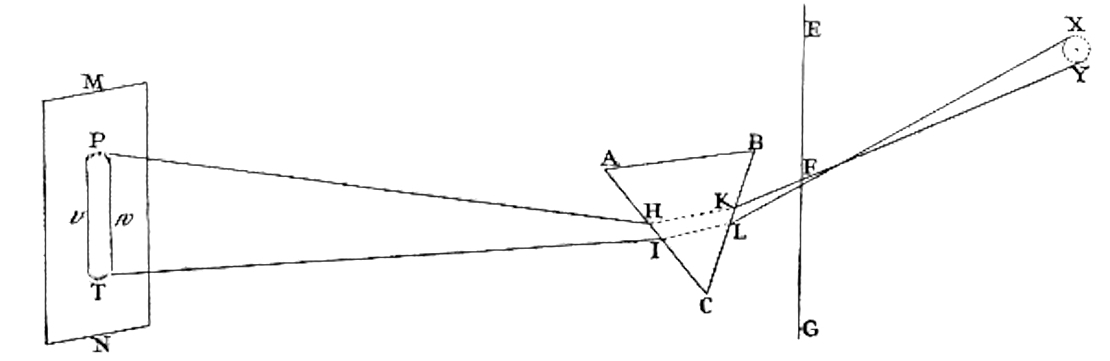
\includegraphics[width=10truecm]{slike/01_Newton.jpg}
\caption{Slika v Newtonovi {\it Optiki} prikazuje razklon sončne svetlobe. Newton 
zapiše, da je razklonjena slika na zaslonu rdeča pri koncu $T$, vijolična
pri koncu $P$, vmes pa rumena, zelena in modra. Vir: https://www.gutenberg.org/}
\label{fig:01_Newton}
\vglue-5truemm
\end{figure}

Pristaš valovnega opisa svetlobe je bil med drugimi Euler\footnote{~Švicarski 
matematik in fizik Leonhard Paul Euler, 1707--1783.}, ki je podal tezo, 
da valovna dolžina valovanja svetlobi določa barvo.\index{Euler, Leonhard}
Ključna dognanja za potrditev valovne teorije je leta 1801 prispeval 
Young\footnote{~Angleški zdravnik in fizik Thomas Young, 1773--1829.}, \index{Young, Thomas}
ko je z interferenčnimi poskusi precej natančno izmeril valovno dolžino 
vidne svetlobe. Na podlagi Huygensovega valovnega pristopa je 
Fresnel\footnote{~Francoski fizik Augustin Jean Fresnel, 1788--1827.} \index{Fresnel, Augustin}
leta 1818 pojasnil interferenčne pojave in izračunal vrsto 
uklonskih slik. Z Aragojem\footnote{~Francoski astronom in fizik
Fran\c{c}ois Jean Dominique Arago, 1786--1853.} sta proučevala \index{Arago, Fran\c{c}ois}
dvolomnost kristalov in interferenco različno odklonjenih žarkov. 
Opazila sta, da med dvema različno polariziranima valovanjema ne 
pride do interference. To je porušilo njuno prepričanje v valovno 
naravo svetlobe, saj so do takrat verjeli, da je svetloba
longitudinalno valovanje. Kar nekaj časa je minilo, preden je Young 
rešil problem s predlogom, da je svetloba transverzalno valovanje.
Kmalu za tem je Fresnel zapisal znane enačbe za jakosti odbitega 
in prepuščenega žarka ob vpadu na mejo med dvema sredstvoma.
Fresnel je v poznejših letih proučeval tudi disperzijo svetlobe.

Okoli 1850 sta se najprej Fizeau\footnote{~Francoski fizik Armand Hippolyte \index{Fizeau, Armand}
Louis Fizeau, 1819--1896.} in pozneje Foucault\footnote{~Francoski fizik
Jean Bernard L\'{e}on Foucault, 1819--1868} lotila natančnega \index{Foucault, Jean}
merjenja hitrosti svetlobe. Prvi je uporabil vrteče nazobčano kolo \index{Hitrost svetlobe}
in več kot $8~\si{\kilo\meter}$ oddaljeno zrcalo. Z močnim svetilom je posvetil med
zobmi kolesa in opazoval svetlobo, ki se je odbila od 
zrcala.\footnote{~Glej npr. Strnad, {\it Fizika, drugi del}, 
DMFA-založništvo (2018).} Opazil je, da se pri določenih kotnih hitrostih 
vrtenja kolesa odbita svetloba ne vrne v izhodišče, saj zadane zob kolesa. 
Na ta način je hitrost svetlobe ocenil na $315\,\,300~\si{km/s}$. Do podobne
vrednosti je prišel tudi Foucault, ki je uporabil eno vrtljivo in eno oddaljeno 
zrcalo. To so bile prve meritve hitrosti svetlobe na Zemlji, zaradi česar
je eksperimentalna postavitev omogočala tudi meritev 
svetlobne hitrosti v snovi. Foucault je leta 1850 nedvomno pokazal, 
da je hitrost svetlobe v snovi manjša od hitrosti svetlobe v zraku, kar je dodatno
potrdilo valovno sliko svetlobe. 

Vzporedno z napredkom optike se je razvijalo tudi področje
elektromagnetizma. Faraday\footnote{~Angleški fizik in kemik Michael Faraday, 1791--1867.} \index{Faraday, Michael}
je leta 1845 ugotovil, da lahko z močnim magnetnim poljem spreminja
smer polarizacije žarka svetlobe. Verjetno najpomembnejše delo
na tem področju je prispeval Maxwell\footnote{~Škotski fizik James Clerk Maxwell, \index{Maxwell, James}
1831--1879.}, ki je v sedemdesetih letih devetnajstega stoletja
zbral in dopolnil znanje o elektromagnetizmu ter zapisal enačbe, ki jih 
danes imenujemo po njem. Na podlagi teh enačb je povsem 
teoretično pokazal, da je splošno elektromagnetno valovanje 
transverzalno. Izračunal je njegovo hitrost in jo
izrazil le s fizikalnimi konstantami. Presenetljivo se je izračunana 
hitrost elektromagnetnega valovanja ujemala 
z izmerjeno hitrostjo svetlobe, zato je Maxwell sklepal, da je svetloba 
elektromagnetno valovanje. Eksperimentalno potrditev je leta
1888 ponudil Hertz\footnote{~Nemški fizik \index{Hertz, Heinrich}
Heinrich Rudolf Hertz, 1857--1894.} z lomom in odbojem elektromagnetnih 
valov. Takrat ni bilo več dvoma -- svetloba je transverzalno 
elektromagnetno valovanje. 

Odprto je ostalo vprašanje, ali svetloba za svoje širjenje \index{eter}
potrebuje snov, tako imenovani eter. Z vprašanjem etra se je 
ukvarjalo veliko raziskovalcev, med drugim Arago, Fresnel, Fizeau, 
\index{Arago, Fran\c{c}ois} \index{Fresnel, Augustin} \index{Fizeau, Armand} 
\index{Airy, Sir George} \index{Lorentz, Hendrik}
Airy\footnote{~Angleški astronom in matematik Sir George Biddell Airy, 1801--1892.} 
in Lorentz\footnote{~Nizozemski fizik in nobelovec Hendrik Antoon Lorentz, 1863--1928.},
vendar je dokončen odgovor podal šele Michelson\footnote{~Ameriški fizik in nobelovec Albert
Abraham Michelson, 1852--1931.} s svojim \index{Michelson, Albert}
interferenčnim poskusom v letih 1881 in 1887. Pokazal je, da
sta hitrosti svetlobe enaki v smeri gibanja Zemlje po prostoru in 
pravokotno nanjo. S tem je dokončno ovrgel obstoj etra in pokazal, 
da elektromagnetno valovanje za širjenje ne potrebuje snovi. 
Einstein\footnote{~Nemški fizik in nobelovec Albert Einstein, 1879--1955.} 
je naredil še korak dlje in trdil, da je hitrost \index{Einstein, Albert}
svetlobe neodvisna od gibanja opazovalca, s čimer je postavil temelje 
teoriji relativnosti. Po dogovoru iz leta 1983 je danes 
hitrost svetlobe  definirana kot $299\,\,792\,\,458~\si{m/s}$. \index{Hitrost svetlobe}

Vrnimo se še enkrat v dvajseta leta devetnajstega stoletja, ko je 
Fraunhofer\footnote{~Nemški fizik Joseph von Fraunhofer, 1787--1826.}\index{Fraunhofer, Joseph von}
proučeval razklon svetlobe na prizmah in uklonskih mrežicah. Izredno
natančna izdelava kakovostnih optičnih naprav mu je najprej omogočila odkritje 
natrijevega dubleta, nato pa opazovanje manjkajočih črt v spektru
svetlobe s Sonca. Pol stoletja je trajalo, da \index{Bunsen, Robert}
sta Bunsen\footnote{~Nemški kemik Robert Wilhelm Eberhard Bunsen, 1811--1899.}
in Kirchhoff\footnote{~Nemški fizik Gustav Robert Kirchhoff, 1824--1887.}\index{Kirchhoff, Gustav}
pojasnila temne črte v spektru z absorpcijo v snovi in postavila temelje
moderne spektroskopije.

Na podlagi Kirchhoffovega dela je Planck\footnote{~Nemški fizik in nobelovec
Max Karl Ernst Ludwig Planck, 1858--1918.} ob prelomu stoletja\index{Planck, Max}
proučeval sevanje črnega telesa. Po več poskusih, ki se niso
ujemali z eksperimentalnimi opažanji, je predlagal povsem novo rešitev problema
v obliki kvantizirane energije elektromagnetnega polja. Na osnovi
Planckove teorije je Einstein oživel delčni model svetlobe, pri čemer
je privzel, da je svetloba sestavljena iz kvantov energije, kasneje 
poimenovanih fotoni. Z Einsteinovo razlago fotoefekta je bila dokončno
potrjena kvantna narava svetlobe. Danes svetlobo obravnavamo
dualno: kot valovanje, ki pojasni interferenčne 
pojave, in hkrati kot delce, ki pojasnijo fotoefekt.
